\chapter{Methods}
The following chapter will analyse the methods used to answer the research questions. Several topics will be discussed, such as literature review, use case evaluation, prototyping, usability tests, and performance analysis.

\section{Literature review}
In the literature review, we extensively analysed existing research, academic articles, and documentation related to zero-knowledge proofs, \ac{NFT}s, Ethereum, and associated technologies. This review provided a solid foundation for understanding state of the art and identifying areas where our research could contribute to developing and applying zero-knowledge proofs in the context of \ac{NFT}s.

\section{Use case evaluation}
In this study, the use case focused on enabling users to present ownership of an \ac{NFT} (Non-Fungible Token) while preserving their privacy. The evaluation assessed the feasibility, requirements, and potential challenges of the developed solution in this specific scenario.

The primary objective of the use case was to design and implement a system that allowed users to prove ownership of an \ac{NFT} without revealing any unnecessary information about themselves or their holdings. The evaluation involved examining existing solutions and techniques, such as zero-knowledge proofs, to determine their suitability. Additionally, the review considered the potential constraints and limitations of the underlying technologies, such as the Ethereum blockchain, and their impact on the system's performance, usability, and security.

The use case evaluation involved the following steps:
\begin{enumerate}
    \item Identifying the requirements: The essential features and functionalities that the system needed to provide to fulfil its purpose were defined. This included privacy, security, ease of use, and compatibility with existing \ac{NFT} standards and blockchain platforms.
    \item Analysing potential solutions: Various technologies, techniques, and approaches were investigated to meet the identified requirements. This involved reviewing the literature on zero-knowledge proofs, examining existing implementations, and evaluating their pros and cons in the use case context.
    \item Assessing feasibility: The practicality and achievability of the proposed solution, given the existing knowledge, resources, and constraints, were determined. This included evaluating the complexity of implementing the solution, the potential impact on system performance and scalability, and the level of expertise required to develop and maintain the system.
    \item Identifying challenges and limitations: The potential obstacles, risks, and drawbacks of the proposed solution were recognised. This involved considering the system's legal, ethical, and social implications, as well as potential vulnerabilities and attack vectors that could compromise its privacy and security guarantees.
    \item Proposing improvements and refinements: Based on the findings of the use case evaluation, modifications or enhancements to the developed solution were suggested to address the identified challenges and limitations and better meet the use case's requirements.
\end{enumerate}

\section{Prototyping}
This chapter will explain the process undertaken to implement the application. The agile methodology (SCRUM using Kanban) was employed in an iterative process to develop the application. The initial stage involved drafting a UI to analyse all the necessary functionalities. Once the mock-up demonstrated all the requirements, an architecture diagram mapping these requirements was created. Following this, the primary focus was developing the smart contract with the required implementation. After completing the smart contract, the frontend and backend were designed to interact with it. User testing commenced when the application was functional as an MVP, leading to multiple iterations and refinements until the product was polished.

\subsection{UI Prototyping}
The first iteration of the draft was done on paper, as the goal was to consolidate all ideas in one place quickly. By analysing the sketch, the MVP requirements and minimum functionalities were identified. Once these were analysed, potential pain points for users when using the application were noted. After addressing possible pain points, the layout was transferred to Figma (a design tool) as a low-fidelity prototype and presented to UX/UI experts for further analysis and potential improvements before development. The implementation began once these steps were completed, setting the stage for a refined and user-friendly application.

\subsubsection{Paper Draft}
The first iteration aimed to capture all possible user journeys through the application, focusing on the primary user interactions.

The paper drafts illustrate the following:
\begin{enumerate}
    \item Figure \ref{Abb3}: Displays the landing page, where users can view all events available in the application.\\
    \begin{figure}[H]
    \centering
    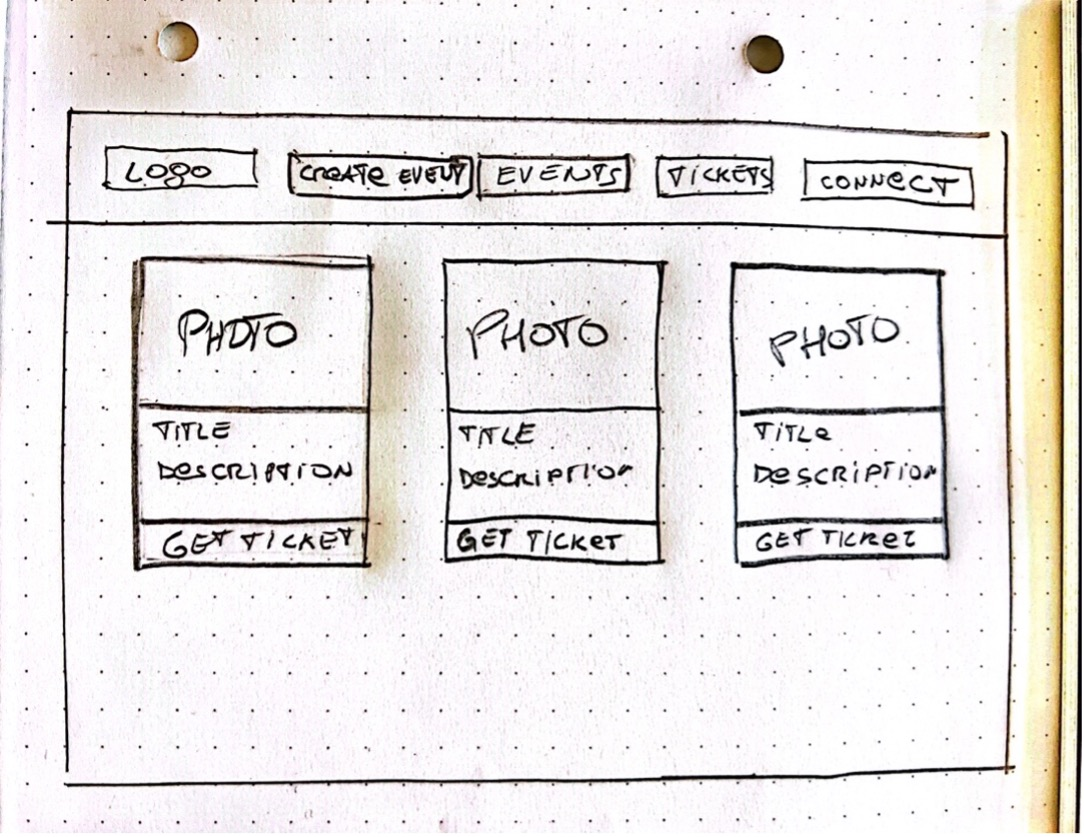
\includegraphics[width=1\linewidth]{PICs/Picture1.jpg}
    \caption{Paper draft of the landing}\label{Abb3}
    \end{figure}
    
    \item Figure \ref{Abb4} Shows the page where users can create events.\\
    \begin{figure}[H]
    \centering
    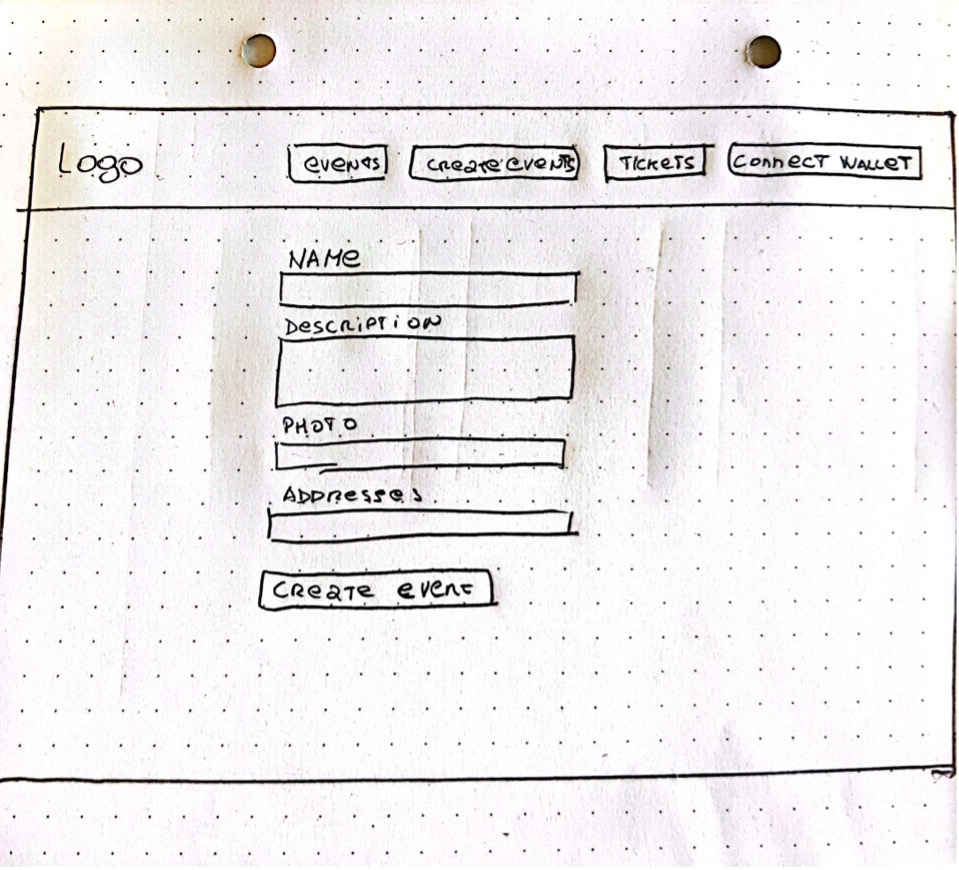
\includegraphics[width=1\linewidth]{PICs/Picture2.jpg}
    \caption{Paper draft of event creation page}\label{Abb4}
    \end{figure}
    
    \item Figure \ref{Abb5}: Portrays the page where users can view their tickets.\\
    \begin{figure}[H]
    \centering
    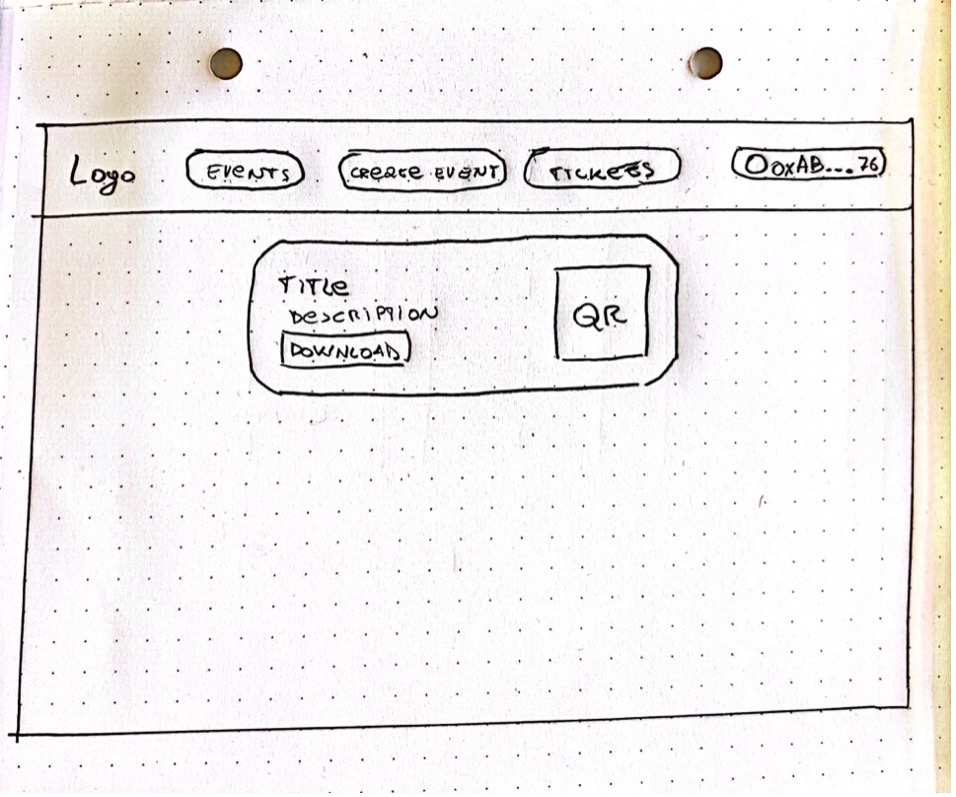
\includegraphics[width=1\linewidth]{PICs/Picture3.jpg}
    \caption{Paper draft of tickets page}\label{Abb5}
    \end{figure}
    
    \item Figure \ref{Abb6}: Displays the view of a bouncer attempting to verify a ticket.\\
    \begin{figure}[H]
    \centering
    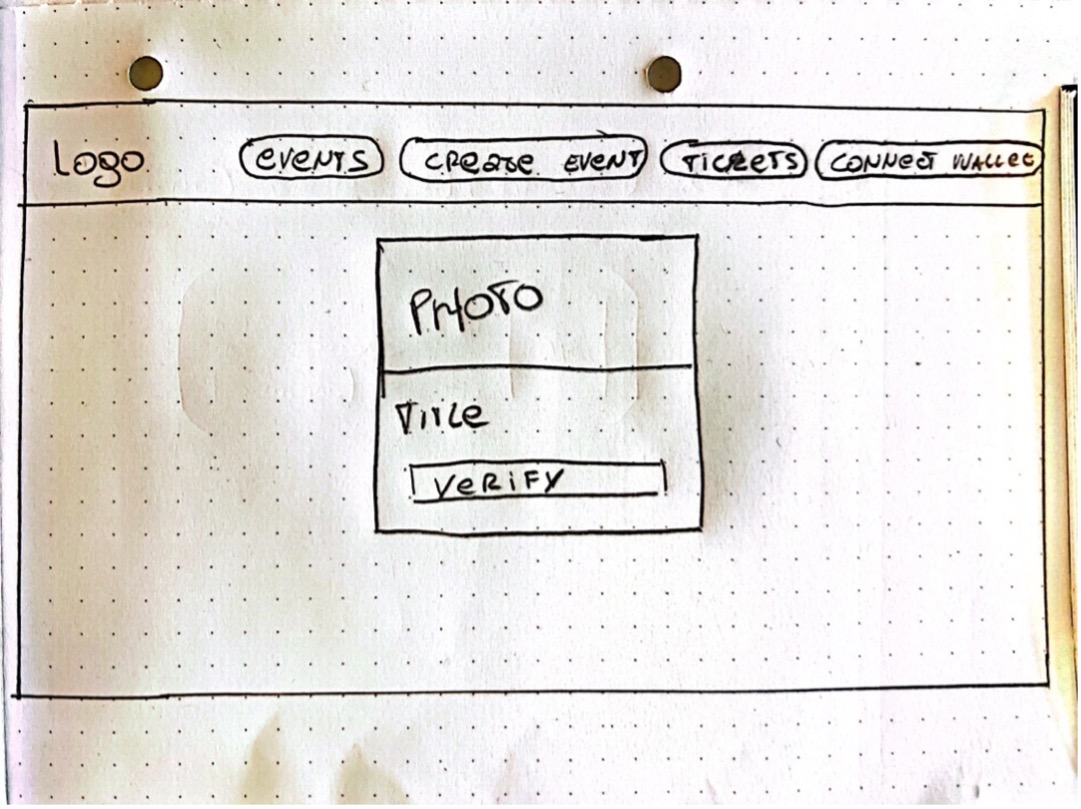
\includegraphics[width=1\linewidth]{PICs/Picture4.jpg}
    \caption{Paper draft of the ticket verification page}\label{Abb6}
    \end{figure}
\end{enumerate}

These paper drafts provided the foundation for the user interface design and allowed me to analyze and refine the user experience before moving on to the following prototyping stages.

\subsection{Low-fidelity Draft}
In this stage, the paper drafts created earlier (as shown in Figures 1-4) were transformed into low-fidelity digital wireframes. The primary goal of developing low-fidelity drafts was to establish the basic structure and layout of the application while keeping a strong focus on usability and user interactions. This approach allowed for quick iterations and modifications as needed, without spending too much time on the visual design elements.

The low-fidelity drafts cover the following aspects:

\begin{enumerate}
\item Figure \ref{Abb7}: Presents a digital wireframe of the landing page, showcasing the list of available events and providing a clearer understanding of the interface elements and navigation. \
\begin{figure}[H]
\centering
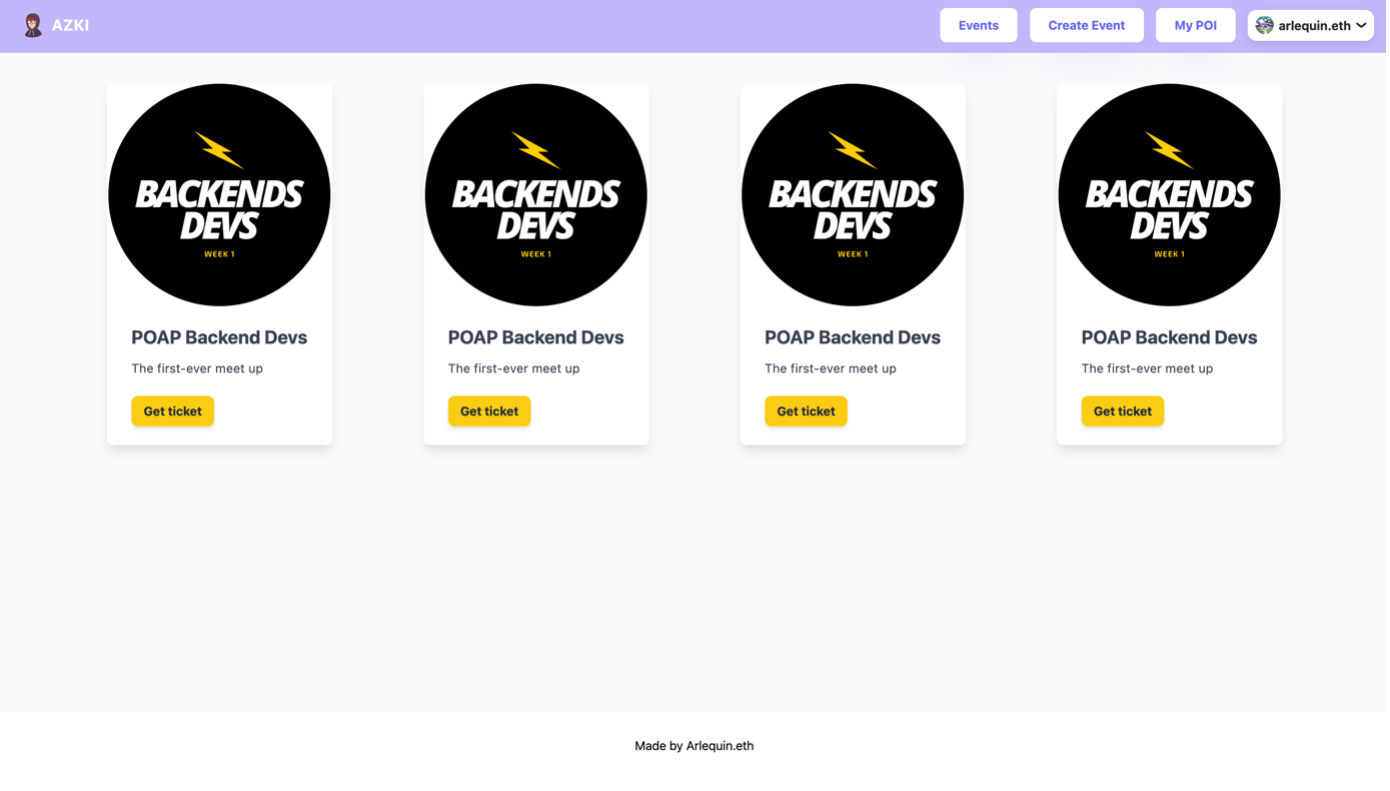
\includegraphics[width=1\linewidth]{PICs/LowFiLanding.png}
\caption{Low-fidelity draft of the landing page}\label{Abb7}
\end{figure}

\item Figure \ref{Abb8}: Illustrates the digital wireframe for the event creation page, highlighting the essential input fields and options required to create an event.\\
\begin{figure}[H]
\centering
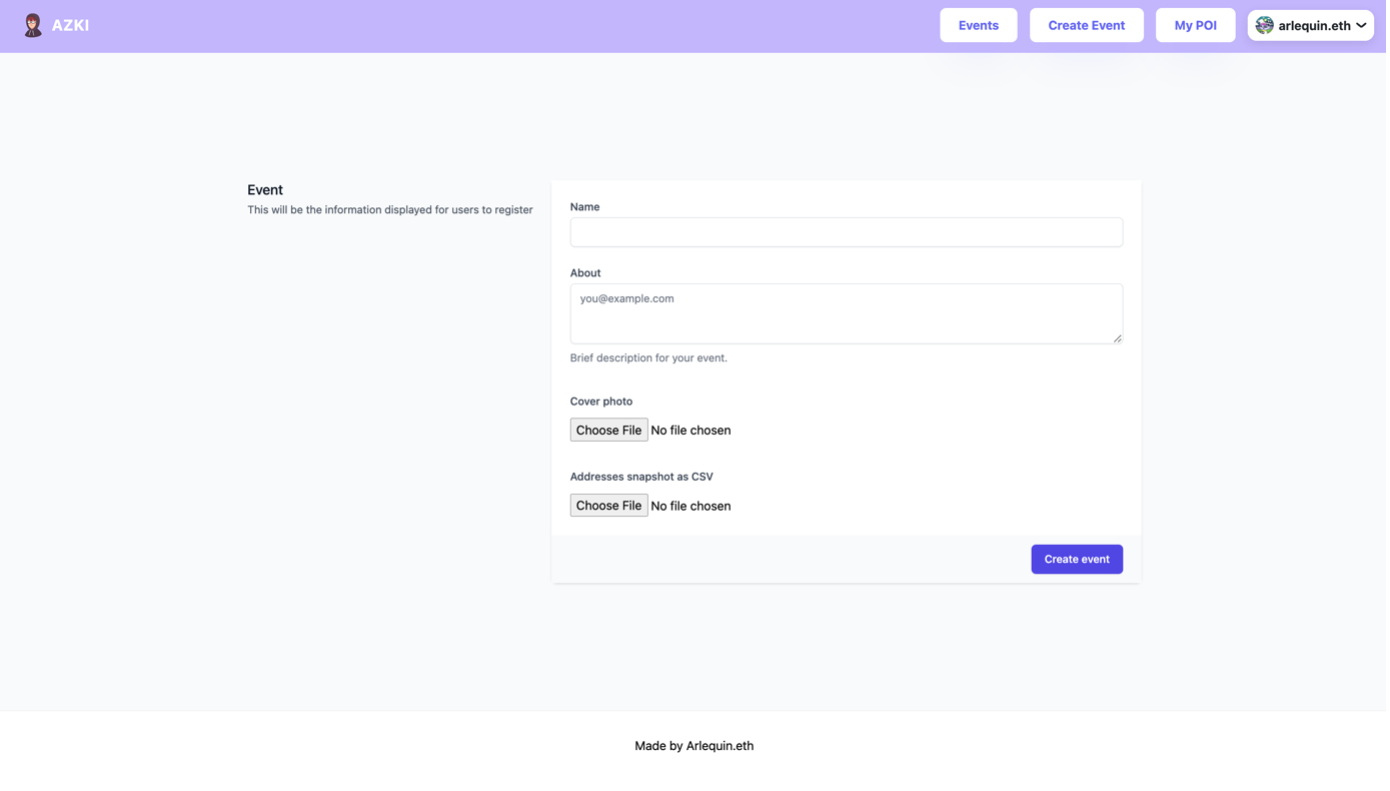
\includegraphics[width=1\linewidth]{PICs/LowFiCreate.png}
\caption{Low-fidelity draft of event creation page}\label{Abb8}
\end{figure}

\item Figure \ref{Abb9}: Depicts the digital wireframe for the tickets page, showcasing the user's ticket collection and relevant information.\\
\begin{figure}[H]
\centering
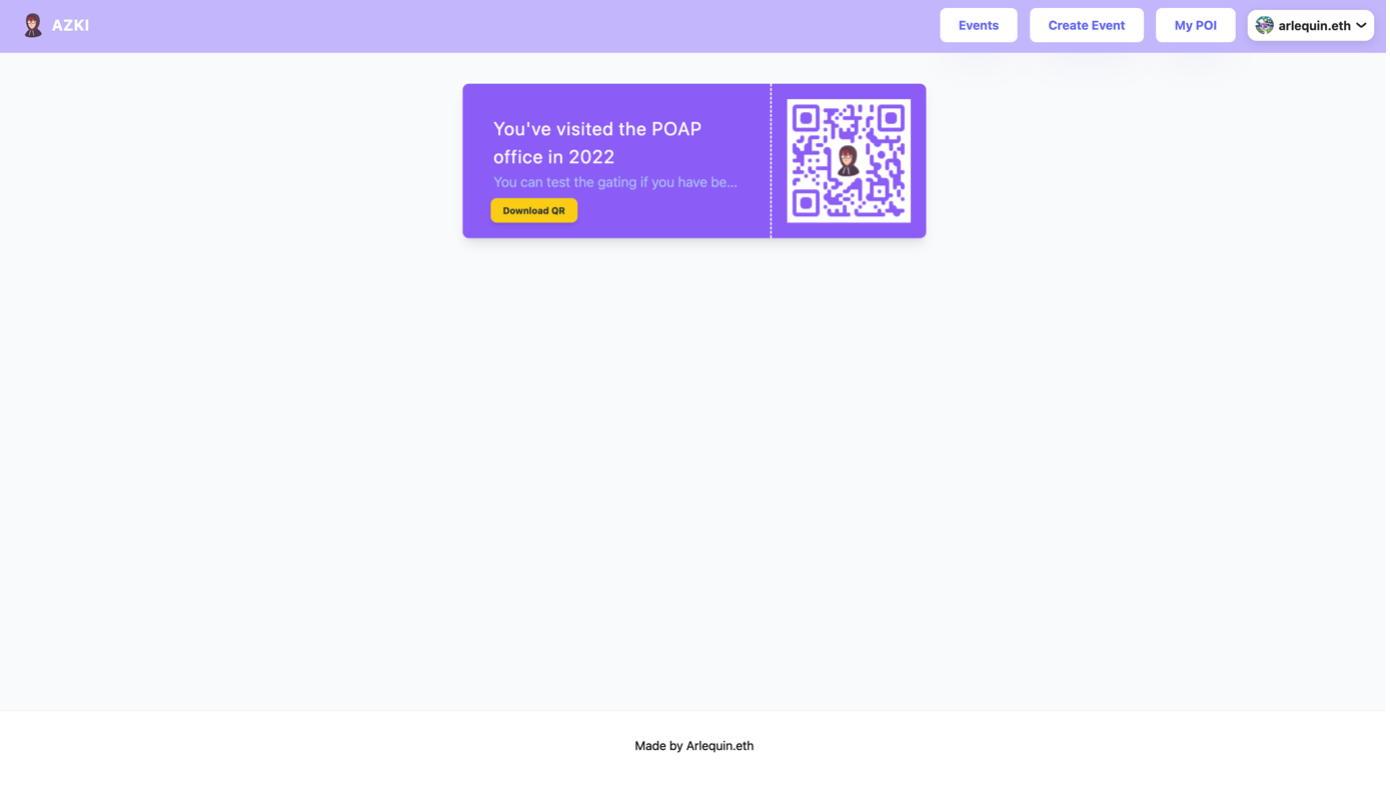
\includegraphics[width=1\linewidth]{PICs/LowFiTicket.png}
\caption{Low-fidelity draft of tickets page}\label{Abb9}
\end{figure}

\item Figure \ref{Abb10}: Demonstrates the digital wireframe for the ticket verification page, focusing on the interaction between the bouncer and the ticket holder during the verification process.\\
\begin{figure}[H]
\centering
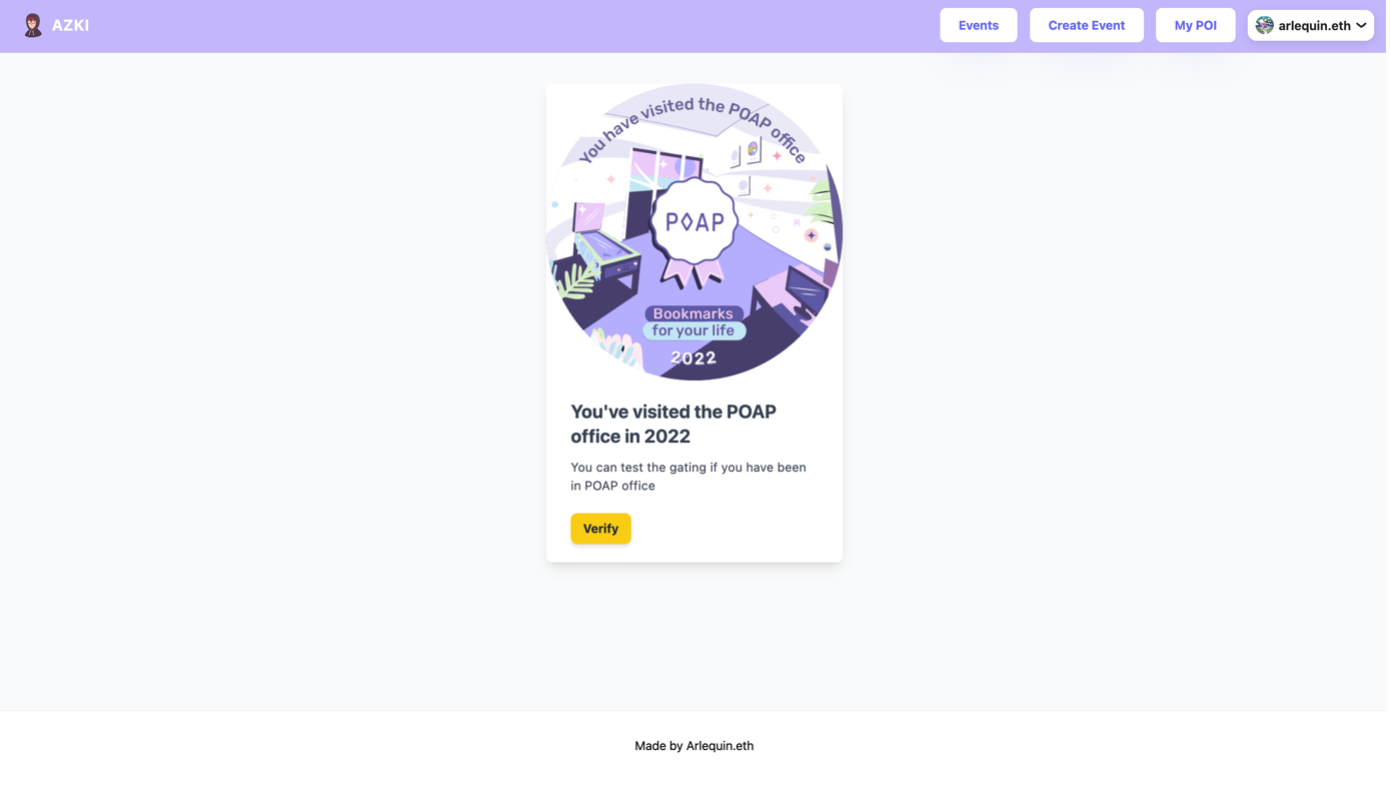
\includegraphics[width=1\linewidth]{PICs/LowFiVerification.png}
\caption{Low-fidelity draft of the ticket verification page}\label{Abb10}
\end{figure}
\end{enumerate}

These low-fidelity drafts served as a crucial step in identifying potential usability issues and refining the user experience. The drafts facilitated iterative improvements and provided a solid foundation for the subsequent development of high-fidelity prototypes.

\subsection{High-fidelity Draft}

After refining the user experience and interactions through the low-fidelity drafts, the next step was to create high-fidelity drafts. These drafts represent the final design of the user interface, incorporating visual elements, typography, color schemes, and detailed interactions. The high-fidelity drafts aimed to create a realistic representation of the final application and facilitate a comprehensive understanding of the user experience.

The high-fidelity drafts encompass the following:

\begin{enumerate}
\item Figure \ref{Abb11}: Showcases a detailed design of the landing page, including the visual elements, color schemes, and typography that contribute to the overall aesthetics of the application. \
\begin{figure}[H]
\centering
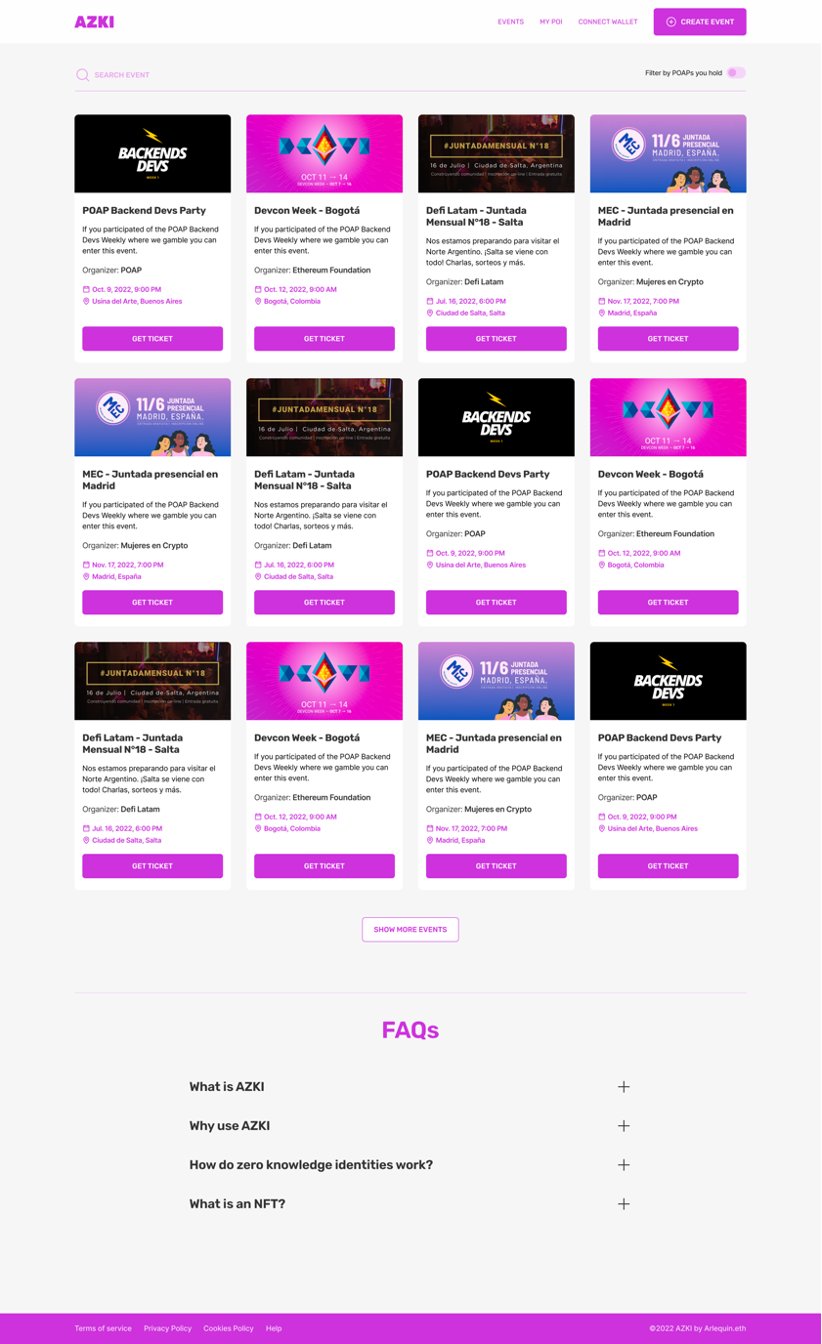
\includegraphics[width=0.8\linewidth]{PICs/HiFiLanding.png}
\caption{High-fidelity draft of the landing page}\label{Abb11}
\end{figure}

\item Figure \ref{Abb12},\ref{Abb13} and \ref{Abb14}: Presents the high-fidelity design for the event creation page, incorporating all necessary input fields and options while maintaining a visually appealing and user-friendly interface.\\
\begin{figure}[H]
\centering
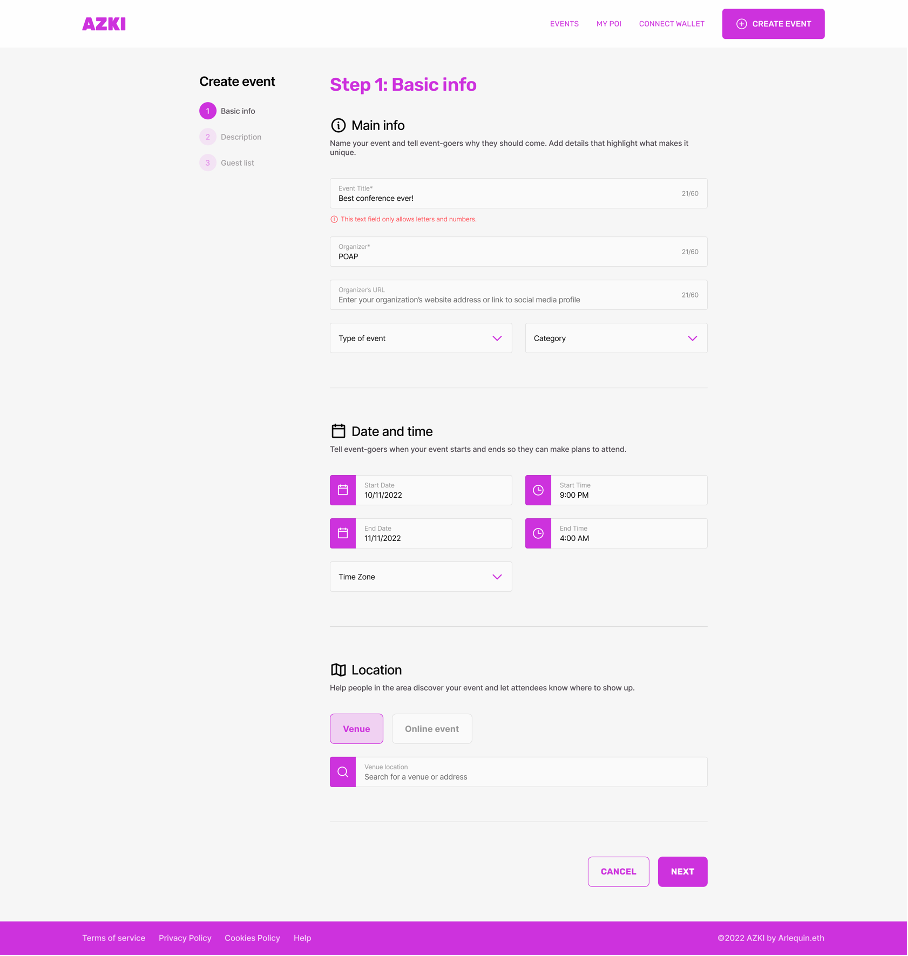
\includegraphics[width=0.8\linewidth]{PICs/HiFiEventCreation.png}
\caption{High-fidelity draft of event creation page}\label{Abb12}
\end{figure}

\begin{figure}[H]
\centering
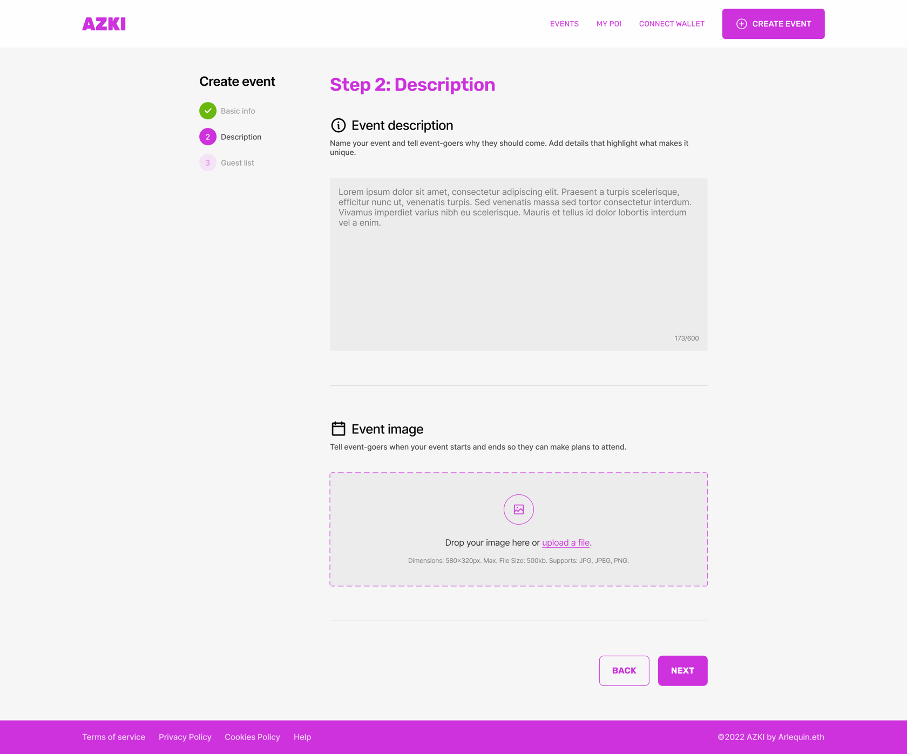
\includegraphics[width=0.8\linewidth]{PICs/HiFiEventCreation2.png}
\caption{High-fidelity draft of event creation page}\label{Abb13}
\end{figure}


\begin{figure}[H]
\centering
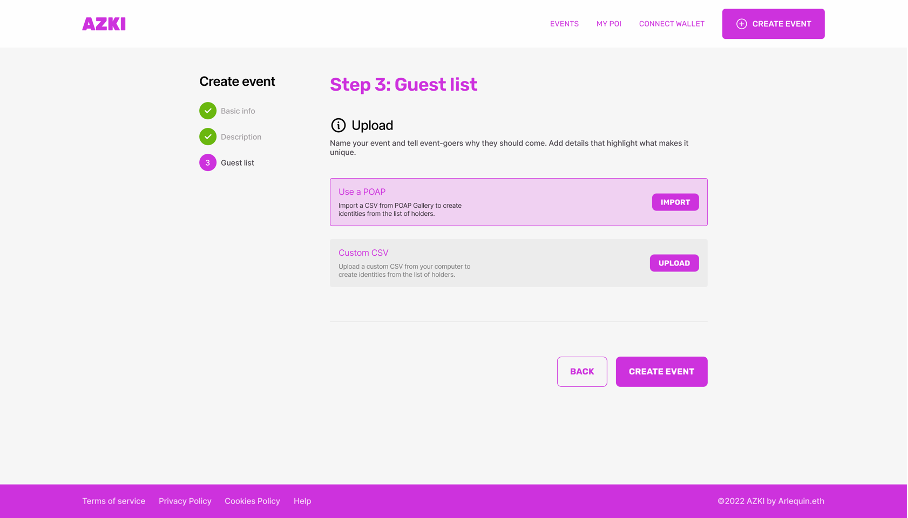
\includegraphics[width=0.8\linewidth]{PICs/HiFiEventCreation3.png}
\caption{High-fidelity draft of event creation page}\label{Abb14}
\end{figure}


\item Figure \ref{Abb15}: Depicts the high-fidelity design for the tickets page, emphasizing the presentation of ticket information and allowing users to easily access and manage their tickets.\\
\begin{figure}[H]
\centering
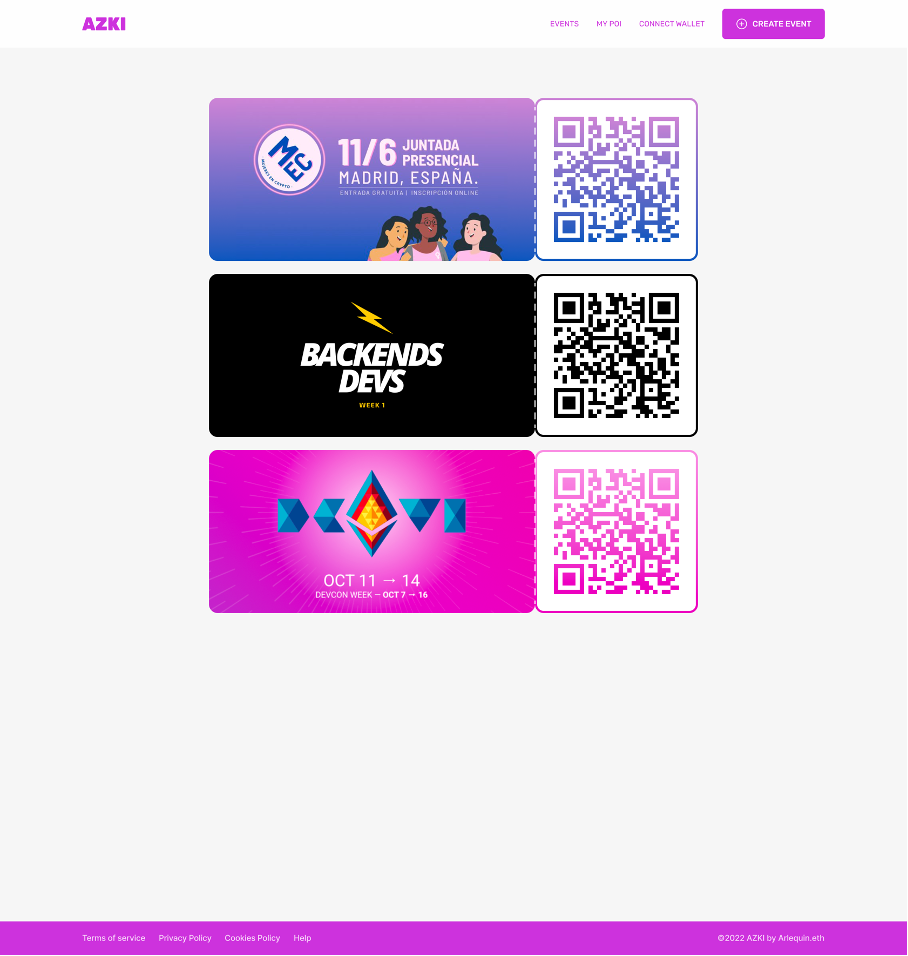
\includegraphics[width=0.8\linewidth]{PICs/HiFiTickets.png}
\caption{High-fidelity draft of tickets page}\label{Abb15}
\end{figure}

\end{enumerate}

The high-fidelity drafts provided a clear and accurate representation of the final application, allowing for the validation of design choices and the assessment of the overall user experience. These drafts played a vital role in bridging the gap between the design and development phases, ensuring that the end product met user needs and expectations.

\section{Architecture}
Once the sketches were completed, the analysis of the architecture began. The project was expected to undergo several iterations, and some aspects of the proposed architecture were considered. The first decision was to utilise a cloud provider to enhance development speed, leading to adopting a \ac{PaaS} called Vercel, which allows frontend and backend deployment with \ac{CI/CD} integration. Another challenge was the uncertainty of the data to be stored in the application, which led to the choice of a document database like Cloud Firestore \cite{google2020cloud_firestore}. Cloud Firestore is a \ac{PaaS} that quickly provides a production-ready database without any overhead for the developer.

For the frameworks, Typescript was chosen because it allows for managing the entire stack with a single language. The front and backend were developed using the Next.js framework, which supports building applications with \ac{SSR}. Solidity was used for the smart contract, as the chosen network was Ethereum.

Considering the importance of security in smart contracts, all functions were tested and had ninety per cent coverage. The libraries zk-kit, circomlibjs, and Ethereum-libs were used to integrate with zero-knowledge. The development was simplified by building contracts on top of Hardhat, allowing for local blockchain testing and easy deployment to the blockchain. OpenZeppelin libraries were also utilised to enhance the security of the contracts, as they are responsible for auditing and creating smart contract standards.

In the front end, the wagmi library was used to facilitate integration with the blockchain, wallets, and other components, providing a ready-to-use solution without reinventing the wheel.

The technologies chosen and their goals are as follows:
\begin{enumerate}
    \item Solidity: A programming language for writing smart contracts on the Ethereum network \cite{soliditylang}.
    \item Hardhat: A development environment for compiling, deploying, and testing Ethereum smart contracts \cite{hardhat}.
    \item TypeScript: A superset of JavaScript that adds optional static types used for both frontend and backend development \cite{typescript}.
    \item OpenZeppelin: A library of secure, reusable, and audited smart contracts for the Ethereum network \cite{openzeppelin}.
    \item Ethers: A library for interacting with the Ethereum blockchain \cite{ethers}.
    \item Zk-kit: A library for working with zero-knowledge proofs in Ethereum smart contracts \cite{zkkit}.
    \item Chai: A BDD/TDD assertion library for node and browser testing \cite{chaijs}.
    \item Next.js: A framework for building server-rendered React applications with lambda functions \cite{nextjs}.
    \item Firebase: A backend-as-a-service platform for building web and mobile applications \cite{firebase}.
    \item Ethereumjs-utils: A collection of utility functions for working with the Ethereum blockchain \cite{ethereumjs}.
    \item Circomlibjs: A library for working with circuits and zero-knowledge proofs \cite{circomlib}.
    \item Rainbow kit: A library for connecting to Ethereum wallets \cite{rainbow}.
    \item Wagmi: A library for simplifying frontend interactions with Ethereum \cite{wagmi}.
\end{enumerate}

\begin{figure}[ht]
\centering
\usetikzlibrary{positioning}
\tikzstyle{block} = [rectangle, minimum width=3cm, minimum height=1cm, text centered, draw=black]
\tikzstyle{arrow} = [thick,->,>=stealth]

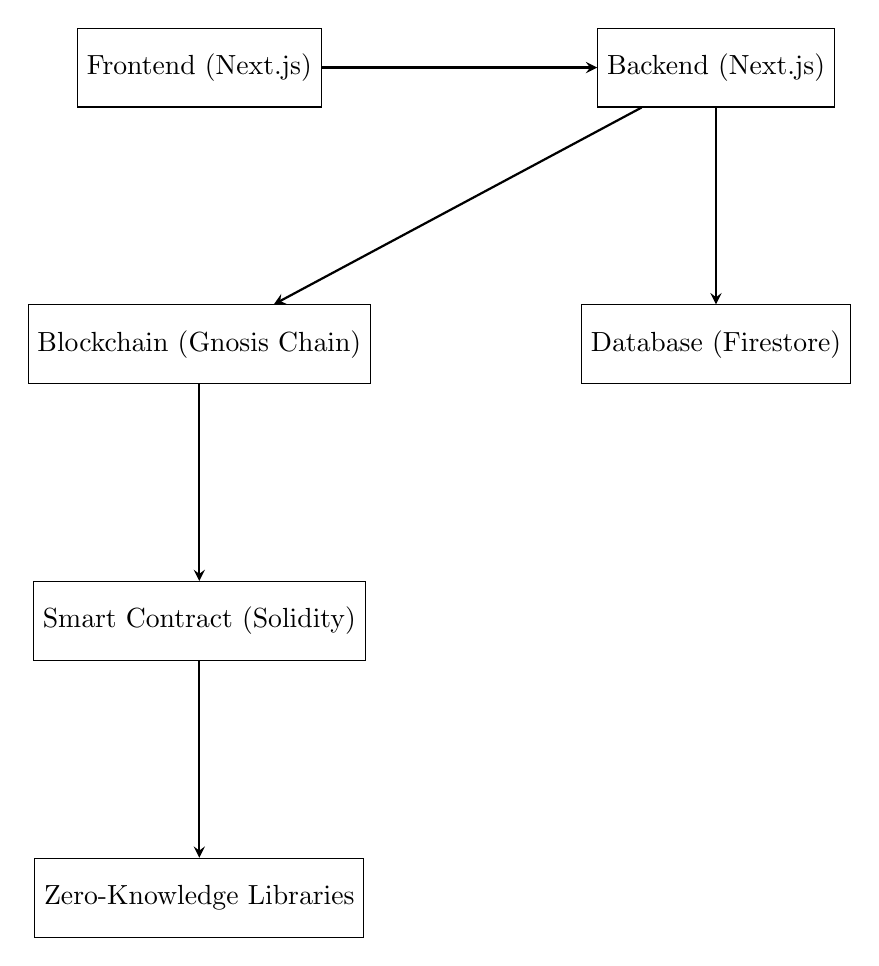
\begin{tikzpicture}[node distance=2.5cm]
\node (frontend) [block] {Frontend (Next.js)};
\node (backend) [block, right=of frontend, xshift=1cm] {Backend (Next.js)};
\node (database) [block, below=of backend] {Database (Firestore)};
\node (blockchain) [block, below=of frontend] {Blockchain (Gnosis Chain)};
\node (smartcontract) [block, below=of blockchain] {Smart Contract (Solidity)};
\node (zklibs) [block, below=of smartcontract] {Zero-Knowledge Libraries};

\draw [arrow] (frontend) -- (backend);
\draw [arrow] (backend) -- (database);
\draw [arrow] (backend) -- (blockchain);
\draw [arrow] (blockchain) -- (smartcontract);
\draw [arrow] (smartcontract) -- (zklibs);
\end{tikzpicture}
\caption{Architecture of the thesis project.}
\label{fig:thesis_architecture}
\end{figure}

The architecture diagram in Figure \ref{fig:thesis_architecture} shows the various components of the thesis project and their relationships. The frontend and backend are both built using Next.js and communicate with each other. The backend interacts with Firestore for data storage and to the Gnosis Chain to interact with the smart contract. The smart contract, written in Solidity, interacts with the zero-knowledge libraries to provide privacy-preserving features.

\section{Frontend}

The frontend of the zk-SNARK based event verification system is built using the Next.js framework, a popular and versatile tool for creating server-rendered React applications. The choice of Next.js allows for efficient development, excellent performance, and easy deployment. This section will discuss the frontend design and implementation, including the user interface, components, and the interaction with the backend.

To enhance the usability of the application, users have the option to retrieve their unique addresses from their POAP (Proof of Attendance Protocol) tokens. This is achieved by associating each event creation with a POAP and its corresponding owner. The addresses required to facilitate this association are obtained from the POAP gallery website \cite{poapWebsite}, which acts as a public record of all POAPs and their respective owners.

\subsection{User Interface}

The user interface is designed to be intuitive and user-friendly, with a focus on simplicity and ease of use. The main components of the UI include:

\begin{itemize}
\item Landing page: Displays a list of all available events and provides options for users to create new events, view their tickets, or log in as a bouncer.
\item Event creation page: Enables users to create new events by entering relevant information such as event name, date, time, and ticket price.
\item Ticket page: Shows the user's purchased tickets and provides options for users to buy additional tickets for available events.
\item Ticket verification page: Allows bouncers to verify the authenticity of a ticket by scanning a QR code or entering a ticket ID.
\end{itemize}

\subsection{Components}

The frontend is composed of several modular React components that can be reused and combined to create the desired user interface. Key components include:

\begin{itemize}
\item EventCard: Represents an individual event in the event list, displaying essential event information and providing options for users to buy tickets.
\item TicketCard: Represents a purchased ticket, displaying the event name, date, and a QR code that can be scanned for verification.
\item EventForm: Provides a form for users to enter event details when creating a new event.
\item VerificationForm: Provides a form for bouncers to enter a ticket ID for manual ticket verification.
\end{itemize}

\subsection{Interaction with Backend and Smart Contracts}

The frontend interacts with the backend server through a combination of RESTful API requests. The following are the key interactions between the frontend and the backend:

\begin{itemize}
\item Fetching event data: The frontend fetches event data from the Firestore database using RESTful API requests to the backend server.
\item Generating zk-SNARK proofs: The frontend requests the generation of zk-SNARK proofs by sending the necessary input data to the backend server, which computes the proofs and returns them to the frontend.
\item Interacting with smart contracts: The frontend interacts with the Gnosis smart contracts using RESTful API requests to the backend server, enabling users to create events, buy tickets, and verify tickets on the blockchain.
\end{itemize}

Overall, the frontend of the zk-SNARK based event verification system is designed to provide a seamless and efficient user experience. By using modern frameworks and libraries, such as Next.js and React, the frontend is highly modular and maintainable, ensuring that it can be easily updated and improved in the future.

\section{Backend}
The backend section of the application plays a crucial role in processing data and managing communication between the front end and the smart contract. It is built using the Next.js framework and uses various libraries and utilities for handling different tasks. This section will discuss the main functions and their roles in the backend component.

\subsection{Fetch Events (GET request)}
This function is responsible for handling GET requests to the /events endpoint. When a GET request is received, the function queries the Firestore database and retrieves the list of event entries. The data is then formatted into an array of objects, including the event ID and all the associated relevant data. The formatted array is then returned as a JSON response.

\begin{lstlisting}[language=Java, name={Fetch Events Function}, label={sc:fetchEvents}]
function handleGetEvents() {
  // Query Firestore for event entries
  const entries = queryFirestore('events');

  // Format event entries into an array of objects
  const formattedEntries = formatEntries(entries);

  // Return formatted entries as JSON response
  return jsonResponse(formattedEntries);
}
\end{lstlisting}

\subsection{Create Event (POST request)}
This function handles the creation of a new event when a POST request is received at the /events endpoint. It starts by extracting the form data, including any attached files, using the formidable library. The function then processes the data, such as uploading the event cover image to the Google Cloud Storage bucket and parsing the CSV file containing participant addresses and identities.
The event's participant addresses are then used to generate zk-SNARK identities using the ZkIdentity library. The generated identities are stored in an array, along with their corresponding addresses. Once all the required data is processed, the function creates a new Firestore document containing the event data and adds it to the events collection.
After the event is created in the Firestore database, the function interacts with the Ethereum smart contract, creating a new event group and adding the participants' zk-SNARK identities to the group.

\begin{lstlisting}[language=Java, name={Create Event Function}, label={sc:createEvent}]
function handlePostEvents(formData) {
  // Process form data and files
  const processedData = processFormData(formData);

  // Generate zk-SNARK identities for participant addresses
  const identities = generateIdentities(processedData.addresses);

  // Create a new event document in Firestore
  createEventDocument(processedData, identities);

  // Interact with Ethereum smart contract
  createEventGroup(processedData, identities);
}
\end{lstlisting}

\subsection{Verify Participant (GET request - /verify)}
This function is responsible for handling GET requests to the /verify endpoint. The function extracts the participant's address from the query parameters and creates a JSON object containing the address and other event details. The JSON object is then base64-encoded and appended to the verification page's base URL. The TinyURL API is used to generate a shortened URL for the verification page, which is then returned as part of the JSON response.

\begin{lstlisting}[language=Java, name={Verify Participant Function}, label={sc:verifyParticipant}]
function handleGetVerify(queryParams) {
  // Extract participant address from query parameters
  const address = extractAddress(queryParams);

  // Create JSON object with address and event details
  const verificationData = createVerificationData(address);

  // Encode verification data and append to verification page base URL
  const verificationUrl = createVerificationUrl(verificationData);

  // Generate shortened URL using TinyURL API
  const shortUrl = generateShortUrl(verificationUrl);

  // Return shortened URL as JSON response
  return jsonResponse(shortUrl);
}
\end{lstlisting}

\subsection{Fetch Event Details (GET request - /events/:id)}
This function retrieves the details of a specific event when a GET request is received at the /events/:id endpoint. The function extracts the event ID from the request parameters and queries the Firestore database to fetch the corresponding event data. The event data is then returned as a JSON response.

\begin{lstlisting}[language=Java, name={Fetch Event Details Function}, label={sc:fetchEventDetails}]
function handleGetEventDetails(eventId) {
  // Query Firestore for event data using the event ID
  const eventData = queryFirestoreById('events', eventId);

  // Return event data as JSON response
  return jsonResponse(eventData);
}
\end{lstlisting}

\subsection{Update Event (PUT request - /events/:id)}
This function updates the details of an existing event when a PUT request is received at the /events/:id endpoint. The function extracts the event ID from the request parameters and the updated event data from the request body. It then updates the corresponding Firestore document with the new event data and returns a JSON response indicating the update's success or failure.

\begin{lstlisting}[language=Java, name={Update Event Function}, label={sc:updateEvent}]
function handlePutEvent(eventId, updatedEventData) {
  // Update Firestore document with new event data
  const updateStatus = updateFirestoreDocument('events', eventId, updatedEventData);

  // Return update status as JSON response
  return jsonResponse(updateStatus);
}
\end{lstlisting}


\subsection{Verify Proof (POST request)}
This function handles the verification of the zk-SNARK proof when a POST request is received at the root endpoint. It extracts the required data from the request body, sets up the Ethereum contract, and attempts to verify the proof. If successful, the function returns a 200 status code, and in case of an error, it returns a 500 status code with an "Unknown error!" message.

\begin{lstlisting}[language=Java, name={Verify Proof Function}, label={sc:verifyProof}]
function handleVerifyProof(req) {
  // Extract required data from request body
  const { groupId, nullifierHash, solidityProof, merkleRoot } = req.body;

  // Set up Ethereum contract and signer
  // ...

  // Attempt to verify proof
  try {
    // Verify proof with the contract
    await contractOwner.verifyProof(groupId, bytes32Signal, nullifierHash, merkleRoot, solidityProof);
    // Return success status
    return res.status(200).end();
  } catch (error) {
    // Return error status and message
    return res.status(500).send("Unknown error!");
  }
}
\end{lstlisting}

\subsection{Generate Proof (POST request)}
This function generates a zk-SNARK proof for a participant when a POST request is received at the root endpoint. It first verifies the participant's Ethereum address by comparing the recovered address from the signed message with the provided address. If the addresses match, it fetches the event details from the Firestore database, generates a zk-SNARK identity, and creates a merkle proof. Finally, it generates a zk-SNARK proof using the Semaphore library and returns the proof, public signals, and event details as a JSON response.

\begin{lstlisting}[language=Java, name={Generate Proof Function}, label={sc:generateProof}]
async function handleGenerateProof(req) {
  // Extract required data from request body
  const { address, message, data, id } = req.body;

  // Verify Ethereum address
  // ...

  // Fetch event details from Firestore database
  const event = await db.collection('events').doc(id).get();
  const eventData = event.data();

  // Generate zk-SNARK identity and merkle proof
  // ...

  // Generate zk-SNARK proof using Semaphore library
  try {
    const { proof, publicSignals } = await Semaphore.genProof(witness, semaphoreWasmPath, semaphoreZkeyPath);
    const solidityProof = await Semaphore.packToSolidityProof(proof);

    // Create response object and return as JSON
    const responseObject = {
      // Event details and proof data
    };
    return res.status(200).json(responseObject);
  } catch (e) {
    // Return error status and message
    return res.status(400).json(e);
  }
}
\end{lstlisting}

These functions, along with the previously mentioned ones, collectively handle the core functionalities of the backend component, ensuring smooth communication between the frontend, Firestore database, and the Ethereum smart contract.



\section{Smart Contract}

A critical aspect of the event management system is the implementation of the smart contract, which is responsible for managing the Proof of Invitation (POI) functionality. The contract oversees the creation and management of user groups, verifies zk-SNARK proofs, and ensures the privacy of participants within the system. In this section, we delve into the smart contract's structure, its core functions, and how it integrates into the event management system.

\subsection{Core Contract}

The core contract is a POI implementation that utilizes the Semaphore library for zero-knowledge proofs. It employs OpenZeppelin's access control features for managing user roles and inherits functionality from Semaphore base contracts, namely SemaphoreCore and SemaphoreGroups. The contract's primary purpose is to manage user groups, add and remove members, and verify zk-SNARK proofs that ensure the privacy of the event participants. You can find the full code in Figure \ref{sc:poiContract}

\subsection{Pseudo Code}

Below is an overview of the primary functions of the POI contract in pseudo code:

\begin{enumerate}
\item Initialize the contract with a Semaphore verifier:
\begin{enumerate}
\item Assign the verifier to the provided address.
\item Establish roles for the contract owner and controller.
\end{enumerate}

\item Manage controllers:
\begin{enumerate}
\item Grant the contract owner the ability to add or remove a controller.
\item Allow controllers to renounce their role.
\end{enumerate}

\item Create a new group:
\begin{enumerate}
\item Restrict group creation to controllers only.
\item Set up the group with a specified ID, Merkle tree depth, and zero value.
\item Emit an event indicating the group's creation.
\end{enumerate}

\item Manage group members:
\begin{enumerate}
\item Allow controllers to add or remove members from a group.
\item Update the group's Merkle tree by adding or removing the member's identity commitment.
\end{enumerate}

\item Verify proofs:
\begin{enumerate}
\item Limit proof verification to controllers only.
\item Validate the existence of the group by checking its root.
\item Utilize the Semaphore verifier to confirm the provided zk-SNARK proof's validity.
\item Store the nullifier hash to prevent double-spending.
\item Broadcast an event upon successful proof verification.
\end{enumerate}
\end{enumerate}

\subsection{Integration with the Event Management System}

The POI contract is integrated into the event management system to facilitate the creation of private events and manage user groups. Users generate zk-SNARK proofs that are verified by the contract to ensure they are valid members of the event. The contract ensures the privacy of participants and prevents unauthorized access to event information.

The smart contract is a crucial component of the event management system, providing the necessary functionality to enforce privacy and manage user groups. The implementation leverages the Semaphore library for zero-knowledge proofs, ensuring a secure and efficient solution for private event management.

\section{Sequence diagrams}
Sequence diagrams provide a visual representation of the interactions between different components in a system. They help in understanding the flow of information and the order of events that occur during the execution of a process. In this section, we will discuss three sequence diagrams that illustrate the key interactions in our application: Event Creation, Request a Ticket, and Verify a Ticket. These diagrams will shed light on the system's architecture and the role of each component in the overall application workflow.

\subsection{Event Creation}
The Event Creation sequence diagram demonstrates the process of creating an event within our application, involving the user, frontend, backend, and the smart contract. This diagram is crucial for understanding how the system creates a new event and adds user identities (in the form of identity commitments) to the event in the Merkle tree structure, ensuring the privacy and security of the user data.

The sequence of events during the event creation process is as follows:
\begin{enumerate}
    \item The user initiates the event creation process by sending a request to the frontend.
    \item The frontend forwards the request, along with the event information and user addresses, to the backend.
    \item The backend then interacts with the smart contract to create the event.
    \item Once the smart contract successfully creates the event, it sends a confirmation back to the backend.
    \item The backend proceeds to add the user identities (in the form of identity commitments) to the event by interacting with the smart contract.
    \item The smart contract adds the identities to the event's Merkle tree and sends a confirmation back to the backend.
    \item The backend informs the frontend that the event has been successfully created.
    \item Finally, the frontend displays a success message to the user, indicating that the event has been created.
\end{enumerate}


\begin{figure}[h]
  \centering
  \begin{sequencediagram}
    \newinst{user}{User}
    \newinst[3]{frontend}{Frontend}
    \newinst[3]{backend}{Backend}
    \newinst[3]{contract}{Smart Contract}

    \begin{call}{user}{Create Event}{frontend}{}
      \begin{call}{frontend}{Send addresses and event info}{backend}{}
        \begin{call}{backend}{Create event}{contract}{}
        \end{call}
        \begin{call}{backend}{Add identities to event}{contract}{}
        \end{call}
        \mess{contract}{Identities added to event in Merkle tree}{backend}
      \end{call}
    \end{call}
    \postlevel
    \mess{backend}{Event Created}{frontend}
    \mess{frontend}{Success Creation}{user}
  \end{sequencediagram}
  \caption{Event Creation Sequence Diagram}
  \label{fig:event_creation_sequence_diagram}
\end{figure}


This sequence diagram helps in understanding the flow of information and the order of events during the event creation process. It also emphasizes the role of each component in creating an event and adding user identities to the event's Merkle tree, ensuring the privacy and security of the user data.

\subsection{Request a ticket}
The Request a Ticket sequence diagram outlines the process by which a user requests a ticket for an event, involving the user, frontend, and backend components of the application. This diagram is essential for understanding the interactions and steps necessary to request a ticket while maintaining the user's privacy.

\begin{enumerate}
  \item The user initiates the ticket request process by interacting with the frontend, asking to get a ticket for a specific event.
  \item The frontend generates a unique message and requests the user to sign it.
  \item The user signs the unique message using their private key and returns the signed message to the frontend.
  \item The frontend sends the signed message and event information to the backend for further processing.
  \item The backend processes the request, generates a ticket for the user's identity, and sends it back to the frontend.
  \item The frontend displays the ticket to the user and saves it locally, ensuring that the user's privacy is maintained throughout the process.
\end{enumerate}

This sequence diagram is useful for understanding the flow of information and the sequence of events during the ticket request process. It also highlights the importance of user privacy, as the signed message ensures that the user's identity remains confidential while requesting a ticket for an event.

\begin{figure}[h]
  \centering
  \begin{sequencediagram}
    \newinst{user}{User}
    \newinst[3]{frontend}{Frontend}
    \newinst[3]{backend}{Backend}

    \begin{call}{user}{Get Ticket}{frontend}{}
      \begin{call}{frontend}{Request to sign unique message}{user}{}
      \end{call}
      \begin{call}{user}{Sign Message}{frontend}{}
      \end{call}
      \begin{call}{frontend}{Send signed message and event info}{backend}{}
        \begin{call}{backend}{Send ticket for that identity}{frontend}{}
        \end{call}
      \end{call}
    \end{call}
    \postlevel
    \mess{frontend}{Show tickets and saves locally}{user}
  \end{sequencediagram}
  \caption{Request a Ticket Sequence Diagram}
  \label{fig:request_ticket_sequence_diagram}
\end{figure}
\subsection{Verify a ticket}
The Verify a Ticket sequence diagram demonstrates the process of verifying a ticket through a series of interactions between the user, frontend, backend, and smart contract components of the application. This diagram is crucial for understanding the steps and interactions required to ensure a ticket is valid and the user's privacy is maintained throughout the verification process.

\begin{enumerate}
  \item The user initiates the ticket verification process by scanning the QR code on their ticket using the frontend application.
  \item The frontend displays a validation page to the user, providing an interface for the user to request ticket validation.
  \item The user requests validation of their ticket's proof by interacting with the frontend validation page.
  \item The frontend sends the user's proof to the backend for further processing and verification.
  \item The backend verifies the proof by interacting with the smart contract responsible for ticket validation.
  \item If the smart contract determines that the proof is valid, it returns a confirmation to the backend.
  \item The backend relays the confirmation to the frontend, indicating that the proof is valid.
  \item The frontend displays a message to the user, informing them that their ticket has been successfully validated.
\end{enumerate}

This sequence diagram is essential for understanding the flow of information and the sequence of events during the ticket verification process. It highlights the importance of maintaining user privacy and ensuring the validity of the proof throughout the ticket validation process.

\begin{figure}[h]
  \centering
  \begin{sequencediagram}
    \newinst{user}{User}
    \newinst[3]{frontend}{Frontend}
    \newinst[3]{backend}{Backend}
    \newinst[3]{contract}{Smart Contract}

    \begin{call}{user}{Scan QR}{frontend}{}
      \begin{call}{frontend}{Show validation page}{user}{}
      \end{call}
      \begin{call}{user}{Request to validate proof}{frontend}{}
        \begin{call}{frontend}{Send proof}{backend}{}
          \begin{call}{backend}{Validates proof}{contract}{}
          \end{call}
        \end{call}
        \mess{contract}{Proof is valid}{backend}
      \end{call}
    \end{call}
    \postlevel
    \mess{backend}{Proof is valid}{frontend}
    \mess{frontend}{Show proof is valid}{user}
  \end{sequencediagram}
  \caption{Verify a Ticket Sequence Diagram}
  \label{fig:verify_ticket_sequence_diagram}
\end{figure}


\section{Usability Tests}
To assess the effectiveness and user-friendliness of the event management system, usability tests were conducted with a diverse group of participants. These tests were designed to evaluate the overall user experience, identify potential areas of improvement, and gather feedback to enhance the system.

\subsection{Set Up}
The usability tests were conducted in a controlled environment with participants using the same device and browser to ensure consistency. Participants were provided with a brief overview of the system, its goals, and an explanation of the zero-knowledge proofs utilized in the system. To minimize potential biases, participants were not given any specific instructions on how to use the system.

\subsection{Study Design}
The study was designed to evaluate the following aspects of the event management system:

\begin{enumerate}
  \item Navigation: Participants were asked to navigate through the system, exploring various features and functionalities. This allowed us to assess the intuitiveness of the interface and the ease with which users could locate and interact with different components.
  \item Task Completion: Participants were given a series of tasks to complete, such as creating an event, uploading participant data, and generating zk-SNARK proofs. This enabled us to evaluate the system's effectiveness in supporting users through these essential processes.
  \item Error Recovery: During the tasks, participants were encouraged to make mistakes and recover from them. This helped us assess the system's ability to guide users through error recovery and provide useful feedback.
  \item Satisfaction: After completing the tasks, participants were asked to rate their overall satisfaction with the system on a scale of 1 to 10. This allowed us to gauge user satisfaction and identify areas that may need improvement.
\end{enumerate}

\subsection{User Persona}
User personas are fictional representations of the target users for a system, created based on research and data about real users. They help to understand the needs, goals, and pain points of the users, enabling designers and developers to create a more user-centered system. In this study, we developed a user persona for the event management system.

To create the user persona, we gathered data from potential users through interviews, surveys, and user testing. We analyzed the data to identify common characteristics, needs, and goals, and used this information to create a fictional character that represents the target user.

\textbf{User Persona: Emily}
\begin{itemize}
\item \textbf{Age:} 34
\item \textbf{Occupation:} Event Planner
\item \textbf{Education:} Bachelor's degree in Business Management
\item \textbf{Goals:}
\begin{itemize}
\item Efficiently manage events while maintaining privacy and security
\item Streamline event planning tasks and save time
\item Improve communication with clients and vendors
\end{itemize}
\item \textbf{Pain Points:}
\begin{itemize}
\item Difficulty keeping track of multiple events and tasks
\item Concerns about data privacy and security
\item Time-consuming manual processes
\end{itemize}
\item \textbf{Technology Use:} Comfortable using web applications and smartphones for professional and personal purposes
\end{itemize}

\subsection{User Journey}
User journeys illustrate the steps a user takes to interact with a system while trying to achieve a specific goal. These journeys help to understand how the user interacts with the system, identify potential issues, and uncover opportunities for improvement. In this study, we created user journeys for the event management system, focusing on the goals and pain points of our user persona, Emily.

\subsubsection{Creating an Event}
\begin{enumerate}
\item Emily logs in to the event management system.
\item She navigates to the "Create Event" page.
\item Emily fills in the event details, such as the event name, date, and location.
\item She selects the privacy settings for the event and uploads the participant data.
\item Emily reviews the information and clicks the "Create Event" button.
\item The system generates zk-SNARK proofs for the participant data, ensuring privacy and security.
\item Emily receives a confirmation message that the event has been created successfully.
\end{enumerate}

\subsubsection{Event Validation}
\begin{enumerate}
\item On the day of the event, John arrives at the venue with his ticket (either digital or printed).
\item A staff member at the entrance uses a QR code scanner or the event management system's validation feature to scan John's ticket.
\item The system verifies the zk-SNARK proof associated with John's ticket, confirming his identity without revealing his personal information.
\item If the validation is successful, the staff member allows John to enter the event.
\item In case of an invalid ticket or a mismatch with the zk-SNARK proof, the staff member denies entry and asks John to contact the event organizer for assistance.
\end{enumerate}

\subsubsection{Claiming a Ticket}
\begin{enumerate}
\item Emily's client, John, receives an email invitation to an event managed by the event management system or searches for the event on the system's website.
\item John clicks on the link in the email or selects the event on the website, which directs him to the event's ticket claim page.
\item John is prompted to log in with MetaMask to confirm his Ethereum address.
\item After logging in and confirming his address, John clicks on the "Claim Ticket" button on the event's ticket claim page.
\item If the claim is successful, John is redirected to a page where he can download his ticket with a unique ticket code and a QR code. He can either save the ticket digitally or print it for event entry.
\item If the claim is unsuccessful, the system displays an error message, such as "Sorry, you cannot claim a ticket for this event." John can then contact the event organizer for assistance.
\end{enumerate}

These user journeys illustrate how Emily interacts with the event management system to achieve her goals, highlighting the system's features and functionalities

\subsection{Data Collection and Analysis}
Data was collected throughout the usability tests, including observations of participants' interactions with the system, their completion times for each task, and any errors encountered. Additionally, participants were asked to provide verbal feedback regarding their experiences, difficulties, and suggestions for improvement.

Following the usability tests, the data was analyzed to identify trends and common issues. This analysis was used to inform potential refinements to the system, with a focus on enhancing user experience and addressing any identified shortcomings.

\section{Performance Analysis}
Performance analysis is an essential aspect of evaluating a software system. It helps in identifying bottlenecks, understanding the system's scalability, and evaluating its overall efficiency. In this section, we will discuss the performance analysis of our zk-SNARK based event verification system, focusing on key metrics such as latency, throughput, and resource utilization.

\subsection{Latency}
Latency refers to the time taken by the system to respond to a request or perform a specific action. In our system, latency can be observed in several operations, such as fetching event data from the Firestore database, generating zk-SNARK proofs, and interacting with the Ethereum smart contract.
To analyze latency, we can measure the time taken for these operations during typical use-cases and identify any performance bottlenecks. The primary factors affecting latency in our system are network delays, database query performance, and the computation time required for zk-SNARK proof generation.
Latency (L) can be calculated as the sum of the time taken to fetch event data ($T_{fetch}$), the time taken to generate zk-SNARK proofs ($T_{proof}$), and the time taken to interact with the Ethereum smart contract ($T_{contract}$). The latency equation is represented as follows:
% Equation for latency
\begin{align}
L = T_{fetch} + T_{proof} + T_{contract}\label{EqLatency}
\end{align}

\subsection{Throughput}
Throughput refers to the number of transactions or operations a system can handle per unit of time. In our system, throughput can be measured by evaluating the number of verifications and proof generations that can be performed concurrently. To analyze the throughput, we can perform load testing by simulating multiple users requesting verifications and proof generations simultaneously.
The factors affecting throughput in our system are the performance of the Firestore database, the efficiency of the zk-SNARK proof generation algorithms, and the Ethereum network's transaction processing capabilities.

Throughput (T) can be measured as the number of verifications ($N_{verifications}$) and proof generations ($N_{proofs}$) performed per unit of time. The throughput equation is given by:
% Equation for throughput
\begin{align}
T = \frac{N_{verifications} + N_{proofs}}{time}\label{EqThroughput}
\end{align}

\subsection{Resource Utilization}
Resource utilization refers to the usage of system resources, such as CPU, memory, and storage, during the execution of the application. Monitoring resource utilization helps in understanding the efficiency of the system and identifying any areas where optimization is required.

To analyze resource utilization, we can use monitoring tools to track the CPU, memory, and storage usage during typical use-cases. The primary factors affecting resource utilization in our system are the efficiency of the Next.js framework, the implementation of the zk-SNARK proof generation algorithms, and the Firestore database's resource consumption.

Resource utilization can be calculated for CPU, memory, and storage usage. The following equations represent the percentage of each resource utilized:

% Equations for resource utilization
\begin{align}
CPU\% = \frac{CPU_{usage}}{CPU_{total}} \times 100\label{EqCPU}
\end{align}

\begin{align}
Memory\% = \frac{Memory_{usage}}{Memory_{total}} \times 100\label{EqMemory}
\end{align}

\begin{align}
Storage\% = \frac{Storage_{usage}}{Storage_{total}} \times 100\label{EqStorage}
\end{align}

These equations help quantify the resource utilization for each of the system's resources, allowing for a better understanding of the system's efficiency and potential areas for optimization.

\subsection{Recommendations for Improvement}
Based on the performance analysis, we can identify areas where optimizations can be made to improve the system's performance. Some recommendations for improvement might include:

\begin{enumerate}
    \item Optimize database queries to reduce latency when fetching event data.
    \item Implement caching strategies to minimize network delays and improve response times.
    \item Optimize the zk-SNARK proof generation algorithms to reduce computation time and resource utilization.
    \item Utilize efficient libraries and tools to minimize the overhead introduced by the Next.js framework.
    \item Investigate alternative blockchain solutions or layer-2 scaling solutions to improve throughput and reduce latency in interacting with the Ethereum smart contract.
\end{enumerate}

By addressing these areas, we can improve the overall performance of the zk-SNARK based event verification system, ensuring a seamless and efficient user experience.

